% ------------------------------------------------------------------
% Q3. Estimation of risk capital
% Requires in the preamble:  \usepackage{graphicx}  \usepackage{booktabs}  \usepackage{amsmath}
% Upload Q3a_BOF1_histogram.png ... Q3e_BOF1_histogram.png to the Overleaf project
% (same folder as the .tex file, or change the paths below).
% ------------------------------------------------------------------

\subsection*{3. Estimation of risk capital}

The SCR is estimated by simulation as the 1-year Value-at-Risk at the 95\% confidence level of the
loss in basic own funds,
\begin{equation*}
  \mathrm{SCR} = \mathrm{VaR}_{0.95}\bigl(-(BOF_1 - BOF_0)\bigr), \qquad BOF_t = A_t - BE_t ,
\end{equation*}
using the 2000 scenarios in \texttt{ScenarioFile.csv}. For each scenario the ALM model is run month by
month up to $t = 12$, where the best estimate $BE_t$ is computed from the 1st order cash flows
discounted with the scenario zero curve at time $t$. At $t = 0$ all scenarios share the same market,
so $A_0 = 2\,100\,000$, $BE_0 = 1\,228\,493$ and $BOF_0 = 871\,507$ for every strategy, and the
duration of the future 1st order cash flows is $D_L(0) = 17.39$ years.

In strategies d) and e) the bond portfolio consists of the rollover bonds Z5 and Z30 (durations 5 and
30 years), with the weight $w_5 = (30 - D_L(t))/25$, truncated to $[0, 1]$, in Z5 so that the bond
duration equals $D_L(t)$. In the CPPI strategy the stock exposure is
$S_t = \min\bigl(\max(2(A_t - BE_t), 0), A_t\bigr)$, i.e.\ multiplier $m = 2$ and floor $BE_t$, which
gives an initial stock share of $2 \cdot BOF_0 / A_0 = 0.83$. All strategies with rebalancing are
rebalanced monthly.

\begin{table}[htbp]
  \centering
  \caption{Basic own funds and SCR (1-year VaR at 95\% of the loss in BOF), 2000 scenarios.}
  \label{tab:q3_scr}
  \begin{tabular}{lrrr}
    \toprule
    Strategy & $BOF_0$ & $\mathrm{E}[BOF_1]$ & SCR \\
    \midrule
    a) BH(0/100)            & 871\,507 &   895\,460 & 211\,985 \\
    b) BH(50/50)            & 871\,507 &   969\,490 & 348\,740 \\
    c) CM(50/50)            & 871\,507 &   968\,366 & 347\,258 \\
    d) CM(50/50), duration  & 871\,507 &   995\,984 & 213\,635 \\
    e) CPPI(2)              & 871\,507 & 1\,044\,325 & 385\,022 \\
    \bottomrule
  \end{tabular}
\end{table}

\begin{figure}[htbp]
  \centering
  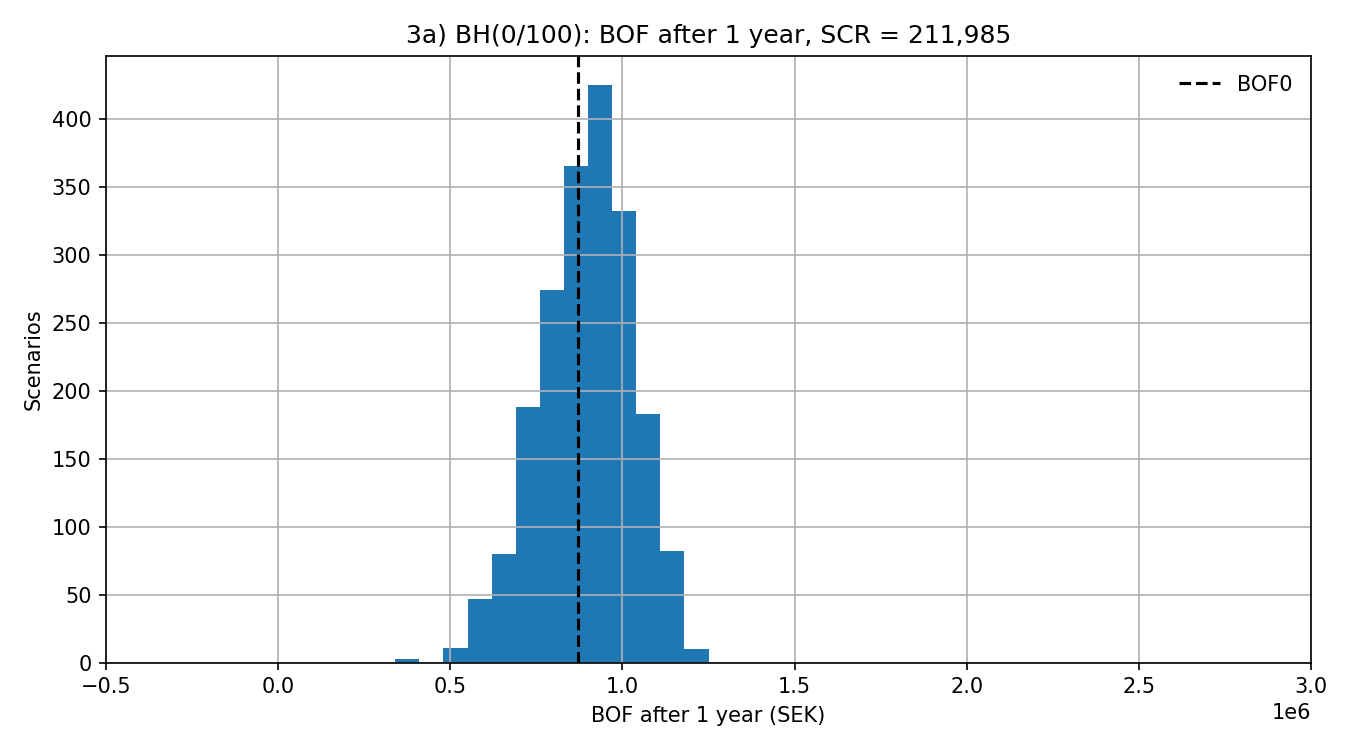
\includegraphics[width=\textwidth]{Q3a_BOF1_histogram.png}
  \caption{3a) BH(0/100): empirical distribution of $BOF_1$ over 2000 scenarios (50 bins), with all
  assets in the Z15 bond. The dashed line marks $BOF_0 = 871\,507$. The distribution is narrow and
  roughly symmetric, with almost all outcomes between about 0.5 and 1.25 million SEK, since the assets
  carry no stock risk and the long bond partly offsets the interest-rate sensitivity of the best
  estimate. SCR $= 211\,985$.}
  \label{fig:q3a}
\end{figure}

\begin{figure}[htbp]
  \centering
  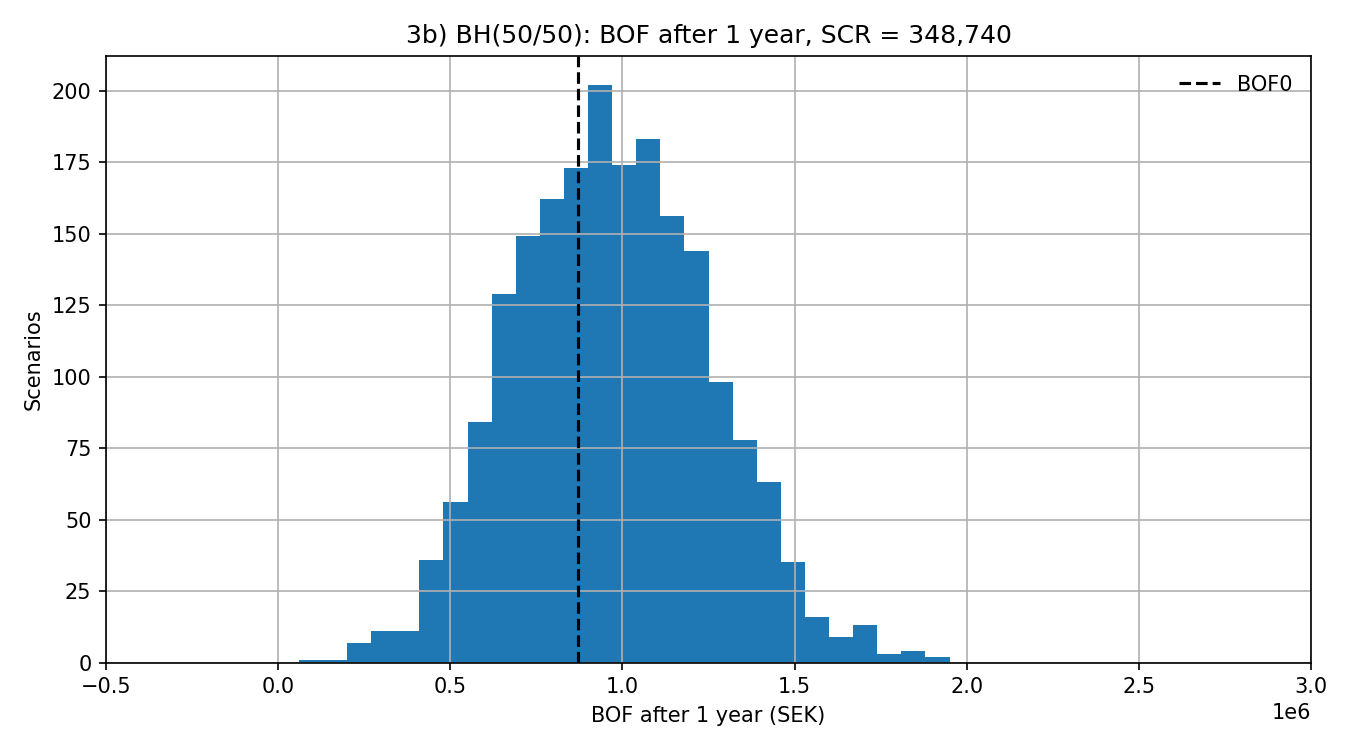
\includegraphics[width=\textwidth]{Q3b_BOF1_histogram.png}
  \caption{3b) BH(50/50): empirical distribution of $BOF_1$ over 2000 scenarios (50 bins), with 50\%
  initially invested equally in the ten stocks and 50\% in Z5, and no rebalancing. The dashed line
  marks $BOF_0 = 871\,507$. The stock exposure makes the distribution much wider than in a), ranging
  from about 0.1 to 1.9 million SEK, with a higher mean ($969\,490$) but also a fatter left tail.
  SCR $= 348\,740$.}
  \label{fig:q3b}
\end{figure}

\begin{figure}[htbp]
  \centering
  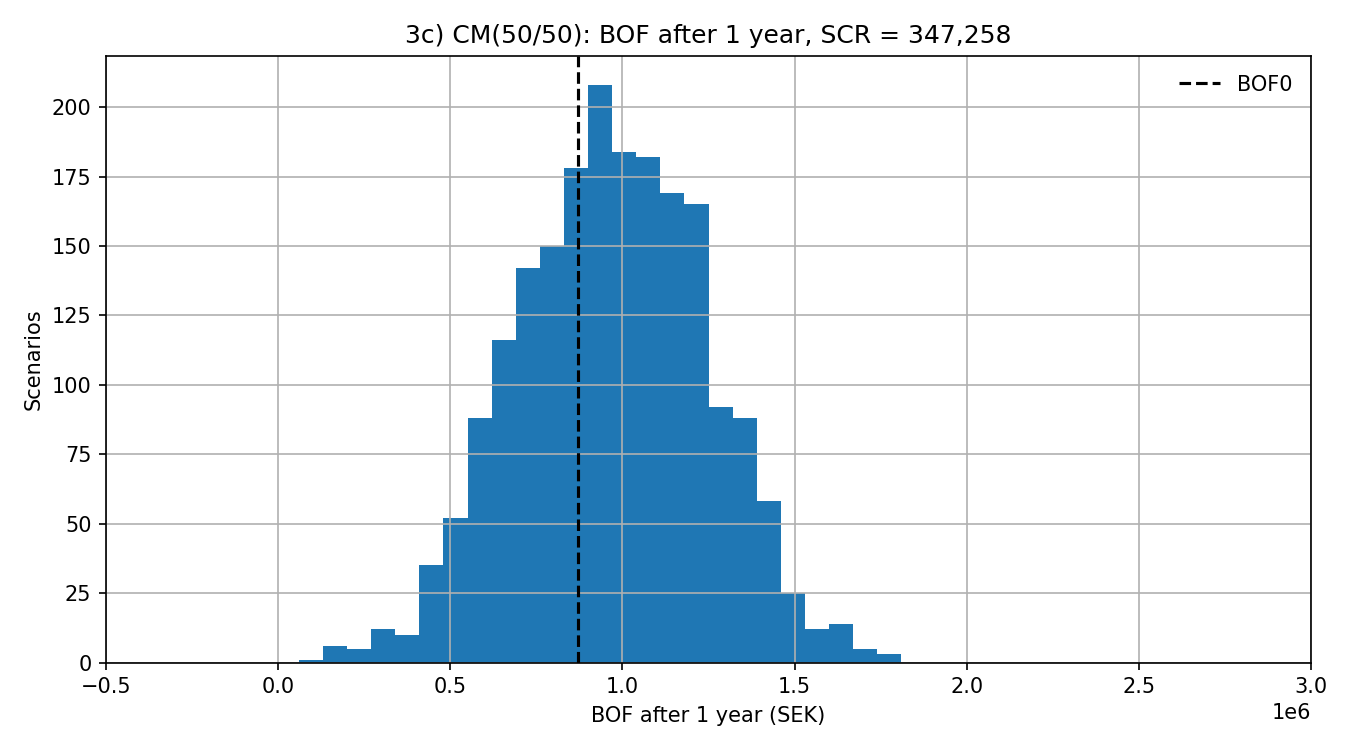
\includegraphics[width=\textwidth]{Q3c_BOF1_histogram.png}
  \caption{3c) CM(50/50): empirical distribution of $BOF_1$ over 2000 scenarios (50 bins), with 50\%
  equally in the ten stocks and 50\% in Z5, rebalanced every month. The dashed line marks
  $BOF_0 = 871\,507$. Over one year the result is very close to the buy-and-hold strategy in b), with a
  similar spread and left tail. SCR $= 347\,258$.}
  \label{fig:q3c}
\end{figure}

\begin{figure}[htbp]
  \centering
  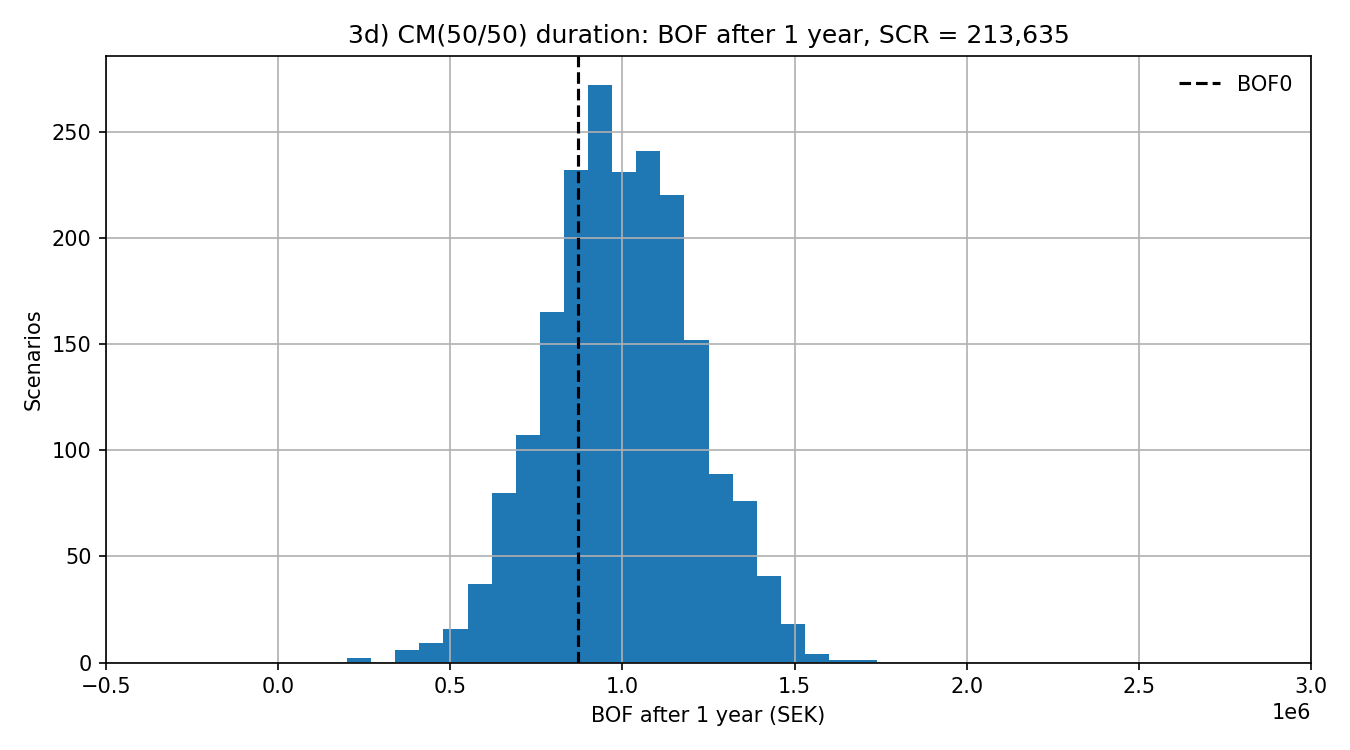
\includegraphics[width=\textwidth]{Q3d_BOF1_histogram.png}
  \caption{3d) CM(50/50) with duration matching: empirical distribution of $BOF_1$ over 2000 scenarios
  (50 bins), with 50\% equally in the ten stocks and 50\% in Z5 and Z30 with duration equal to that
  of the future 1st order cash flows, rebalanced every month. The dashed line marks
  $BOF_0 = 871\,507$. Matching the bond duration to the liabilities hedges most of the interest-rate
  risk, so the distribution is clearly narrower than in b) and c), mostly between about 0.4 and 1.6
  million SEK. SCR $= 213\,635$.}
  \label{fig:q3d}
\end{figure}

\begin{figure}[htbp]
  \centering
  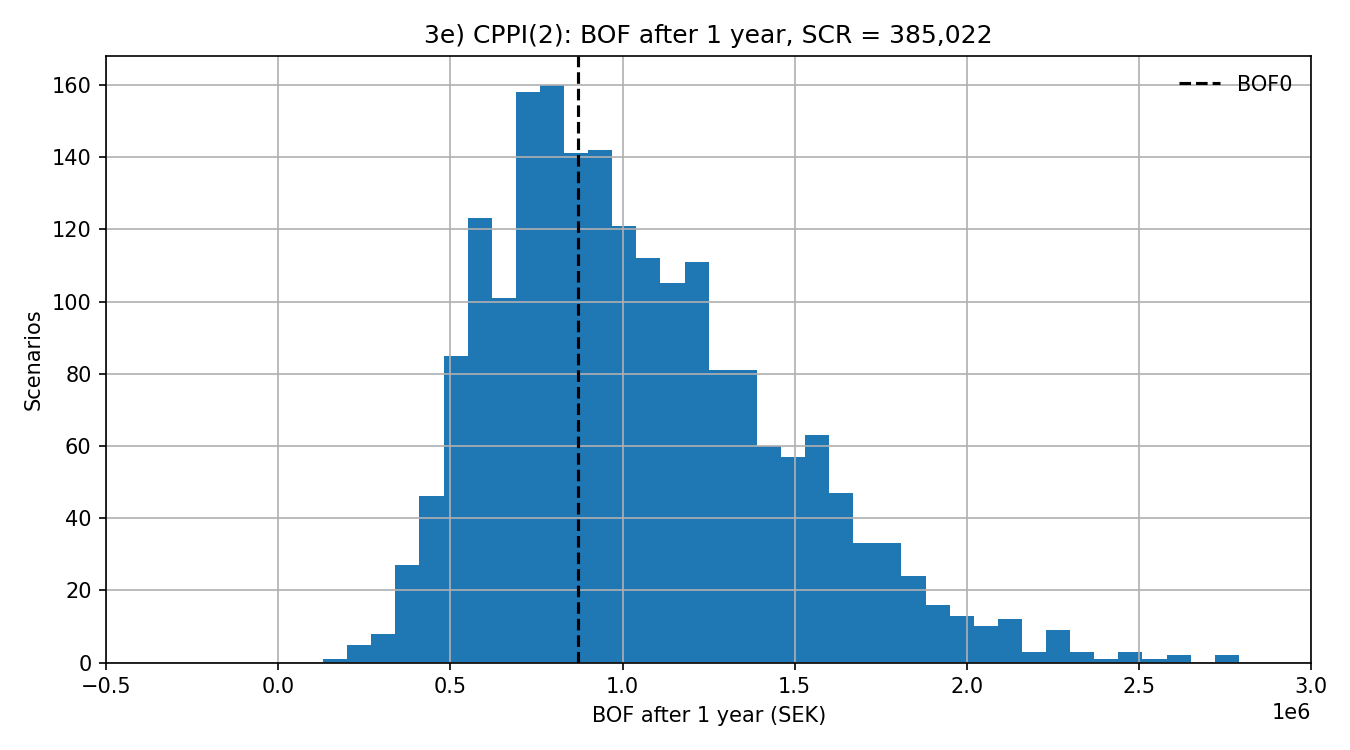
\includegraphics[width=\textwidth]{Q3e_BOF1_histogram.png}
  \caption{3e) CPPI(2): empirical distribution of $BOF_1$ over 2000 scenarios (50 bins), with stock
  exposure $2(A_t - BE_t)$ spread equally over the ten stocks and the rest in Z5 and Z30 with
  duration equal to that of the future 1st order cash flows, rebalanced every month. The dashed line
  marks $BOF_0 = 871\,507$. The distribution is right-skewed, with a long right tail up to about 2.8
  million SEK and the highest mean ($1\,044\,325$). With monthly rebalancing over a single year, the
  high initial stock share (83\%) still gives the largest SCR $= 385\,022$.}
  \label{fig:q3e}
\end{figure}
